\documentclass[12pt, a4paper]{article}

\usepackage{multicol}
\usepackage{geometry}
\usepackage{setspace}
\usepackage{CJKutf8}
\usepackage{amsmath}
\usepackage{listings}
\usepackage{graphicx}

\title{
    \textbf{Report Title} \\
    \large Report Subtitle \\
    \small Tracy Liu
    \author Tracy Liu
    \date{}
}

\geometry{a4paper,left=2cm,right=2cm,top=2.8cm,bottom=3.2cm}
\setlength{\columnsep}{1cm}
\setlength{\baselineskip}{100pt}
\linespread{1.2}
\graphicspath{ {./images/} }

\begin{document}
    \begin{CJK*}{UTF8}{bsmi}

    % title
    \begin{center}
        \LARGE\textbf{2019 Fall Introduction to Operating Systems} \\
        \large Homework 4 \\
        \small 0616015 劉姿利 \\
    \end{center}

    % \begin{multicols*}{2}

    % contents
    \section{hw4\_Series}
        \subsection{Counting the Numbers Locally}
\begin{lstlisting}[language=C++]
for (LL i = L; i < R; i ++) {
    LL num = (int)(input[i] - '0');
    _cnt[num] ++;
}
\end{lstlisting}

        \subsection{Adding the Count into Global Variable}
\begin{lstlisting}[language=C++]
for (LL i = 0; i < 10; i ++) {
    sem_wait(&sem[i]);
    cnt[i] += _cnt[i];
    sem_post(&sem[i]);
}
\end{lstlisting}
        
        \subsection{The Results}
            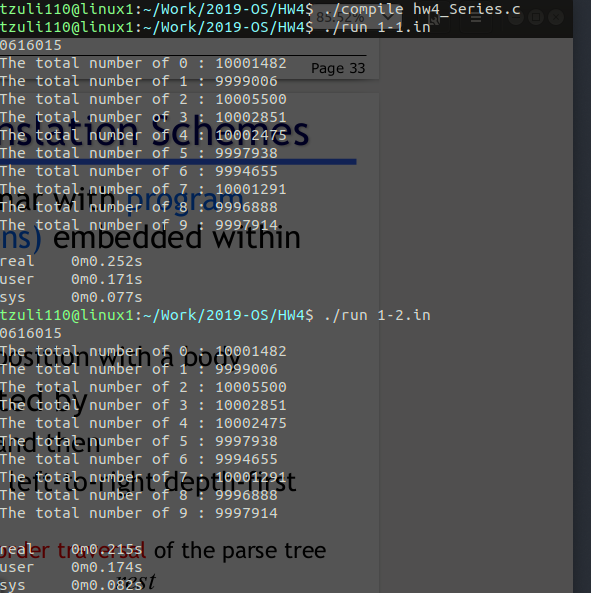
\includegraphics[width=15cm]{series.png}

    \section{hw4\_Pi}

        \subsection{Sample Points}

\begin{lstlisting}[language=C++]
LL _sample = n / k;
while (_sample --) {
    rand_x = (double)(rand_r(&seed) % (INTERVAL + 1)) / INTERVAL;
    rand_y = (double)(rand_r(&seed) % (INTERVAL + 1)) / INTERVAL;
    if (rand_x * rand_x + rand_y * rand_y < 1)
        _cnt ++;
}
\end{lstlisting}

        \subsection{Adding into the Global Variable}
\begin{lstlisting}[language=C++]
sem_wait(&sem);
total += _cnt;
sem_post(&sem);
\end{lstlisting}

        \subsection{The Results}
            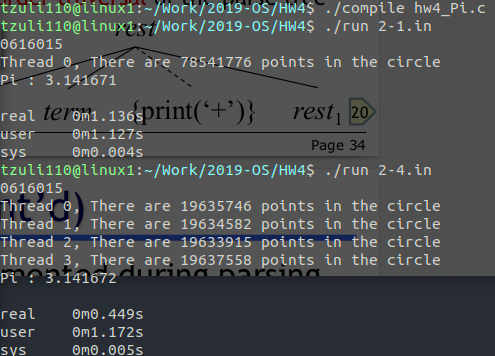
\includegraphics[width=15cm]{pi.png}


    % \end{multicols*}
    \end{CJK*}
\end{document}
